%\newpage

\section{Overhead of a barrier synchronization}
\label{overhead}

There are many ways of implementing a barrier synchronization. In this
paper, we focus on the so-called \emph{centralized barrier}, simply
because in a globally addressed memory system with wide bandwidth
among node processors, such as a POWER4, the centralized barrier will
make the coding much easier, and less error prone\footnote {When there
  is a large number of processor nodes connected by a interconnection
  network with a specific topology, centralized barrier may not be
  preferable. While the barrier in Figure \ref{fig:barriers} (b) will
  be more interesting, where locality is emphasized.}.

Several ways to implement this kind of barrier were suggested in
\cite{Mel91} and re-examined on a ccNUMA system in \cite{Nik99}.
Basically, a shared variable is updated as each thread arrives at the
barrier point. The thread will leave the position if testing finds out
that all the threads have arrived. To understand the overhead of the
whole process, we first have a brief introduction on the 
hardware architecture used for testing, and our test
environment.

\subsection{POWER4 SMP architecture and software}

The basic building block for a POWER4 SMP system can be found in
\cite{Ste01}. It is a multi-chip module (MCM) with four POWER4 chips
forming an 8-way SMP, as shown in Figure \ref{fig:mcm}.  Multiple MCMs
can then be interconnected to form 16-, 24-, and 32-way SMPs.

\begin{figure*}[hbt]
  \begin{center}
    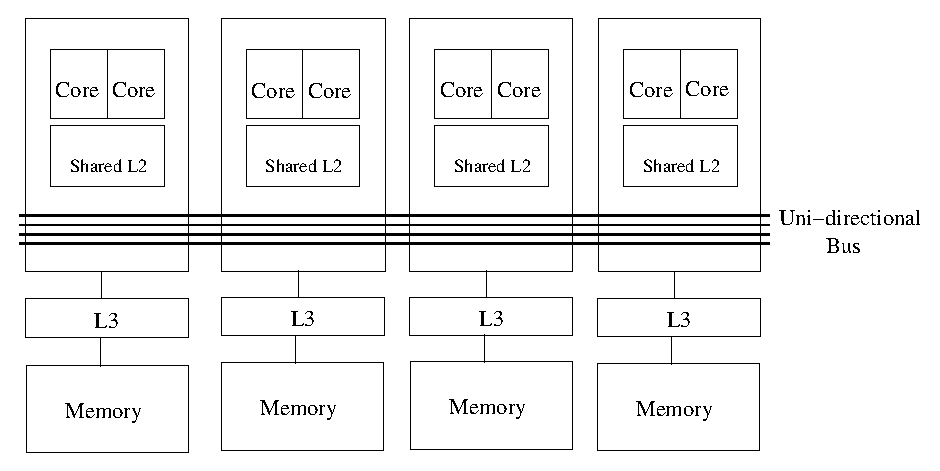
\includegraphics[angle=0, width=0.8\textwidth]{power4mcm.eps}
    \caption{POWER4 MCM structure}
    \label{fig:mcm}
  \end{center}
\end{figure*}

The logical interconnection of four POWER4 chips is point-to-point,
with uni-directional buses connecting each pair of chips to form an
8-way SMP with an all-to-all interconnection topology. The fabric
controller on each chip monitors (for example snoops) all buses and
writes to its own bus, arbitrating between the L2 cache, I/O
controller, and the L3 controller for the bus. Requests for data from
an L3 cache are snooped by each fabric controller to determine if it
has the data being requested in its L2 cache (in a suitable state), or
in its L3 cache, or in the memory attached to its L3 cache. If any one
of these is true, then that controller returns the requested data to
the requesting chip on its bus. The fabric controller that generated
the request then sees the response on that bus and accepts the data.

Up to four MCMs can be interconnected by extending each bus from
each module to its neighboring module in one direction. Inter-module
buses run at half the processor frequency and are 8-bytes wide. The
inter-MCM topology is that of a ring in which requests and data move
from one module to another module in one direction. As with the single
MCM configuration, each chip always sends requests, commands and data
on its own bus but snoops all buses for requests or commands from
other MCMs.

The underlying software system is the SMP runtime library supporting
the OpenMP standard. It is not a research system but production
level software available in the IBM$^{\textregistered}$ 
XL Fortran and VisualAge C++$^{\textregistered}$ products.
The runtime system implements schedule-based barrier synchronization
as well as a fallback for the busy-wait method.

\subsection{Testing benchmark}

We use unmodified EPCC micro-benchmarks to test the performance of a
barrier synchronization. As introduced in \cite{Bul99}, the overhead
here is considered as the difference between the parallel execution
time and the ideal time, given by perfect scaling of the sequential
program.

The parallel execution time is taken from the following code segment, 

%\begin{figure*}[htbp]
%  \begin{center}
{\small
\begin{verbatim}
      dl = delaylength

      do k=0,outerreps
         start  = getclock()
!$OMP PARALLEL  PRIVATE(J)                   
         do j=1,innerreps
            call delay(dl)
!$OMP BARRIER                                
         end do
!$OMP END PARALLEL
         time(k) = (getclock() - start) *
     &             1.0e6 / dble (innerreps)
      end do
\end{verbatim}
% close the $
}
%    \caption{EPCC barrier test}
%    \label{fig:epcctest}
%  \end{center}
%\end{figure*}

While the sequential reference time is measured through this code,

{\small
\begin{verbatim}
      dl = delaylength 
      do k=0,outerreps
         start  = getclock()
         do j=1,innerreps
            call delay(dl)
         end do
         time(k) = (getclock() - start)*
     &             1.0e6 / dble (innerreps) 
      end do
\end{verbatim}
}

In the test program, the value of \texttt{outerreps} is set to 50,
which is the default in the EPCC micro-benchmarks. The array variable
\texttt{time} is used to compute the mean and standard deviation of
the 50 measurements. Since we can exclusively access the machine, only
the mean value is considered here.

\subsection{Barrier overhead on an SMP system}

The two main reasons for the overhead of a barrier synchronization are
memory contention and traffic.  We define \emph{contention} as the effect
produced by many threads accessing simultaneously the same data, and
\emph{traffic} as the amount of data per time unit moving through the
bus. 

Nevertheless, contention and traffic are not independent as some
accesses to memory increase both (so, contention in one memory
position is likely to increase traffic).  Studying memory behavior
through hardware counters can show us an approximation to both the
contention and traffic that a concrete barrier implementation puts on
the system.

In order to reduce the complexity of the analysis, we separate the
barriers into phases:

\begin{itemize}
\item Signaling: Time to enter the barrier and notifying that we are
  in
\item Leaving: Time to realize that the synchronization is over and we
  can leave the barrier
\end{itemize}
This classification can be useful because some implementations focus on 
reducing the impact of the first while others focus on the second. 


%The overall overhead can be calculated, then, as the sum of
%those two times. Decomposition of the barrier in those two times can
%be interesting because in some cases behavior between the two phases
%is significantly different.



